\section{Regularization}

\textbf{Regularization Term:} $\mathcal{R}$ penalizes model complexity. For $\lambda \geq 0$:
\begin{align*}
    h_s & = \arg\min_{h \in \mathcal{H}} F_s(h) + \lambda \mathcal{R}(h)
\end{align*}
\begin{itemize}
    \item $\lambda = 0$: No penalty, may overfit.
    \item $\lambda \to \infty$: Strong penalty, simpler hypothesis.
    \item \textbf{Tradeoff:} Larger $\lambda$ $\rightarrow$ higher bias, lower variance.
    \item \textbf{Where to add regularization:} Add the term where total loss is computed for model selection (usually empirical risk).
    \item \textbf{What to regularize:} Regularize what controls model capacity/flexibility (e.g. weights in neural networks, coefficients in linear models).
\end{itemize}

\subsection{Linear Regression Regularization}
\begin{itemize}
    \item \textbf{L0 Regularization (Best Subset Selection):} Penalizes number of nonzero coefficients.
          \[
              \min_{w_0 \in \mathbb{R},\, w \in \mathbb{R}^d} \left\{ \|w_0 \cdot \vec{1} + Xw - y\|^2 + \lambda \|w\|_0 \right\}
          \]

    \item \textbf{L1 Regularization (Lasso):} Promotes sparsity via absolute value penalty.
          \[
              \min_{w_0 \in \mathbb{R},\, w \in \mathbb{R}^d} \left\{ \|w_0 \cdot \vec{1} + Xw - y\|^2 + \lambda \|w\|_1 \right\}
          \]

    \item \textbf{L2 Regularization (Ridge):} Penalizes large coefficients via squared norm.
          \[
              \min_{w_0 \in \mathbb{R},\, w \in \mathbb{R}^d} \left\{ \|w_0 \cdot \vec{1} + Xw - y\|^2 + \lambda \|w\|_2^2 \right\}
          \]

    \item \textbf{Tikhonov Regularization:} Generalizes Ridge by penalizing $\|Lw\|^2$ for matrix $L \in \mathbb{R}^{k \times d}$.
          \[
              \hat{w}_L^{\text{Tik}} = \arg\min_{w \in \mathbb{R}^d} \left\{ \|Xw - y\|^2 + \|Lw\|_2^2 \right\}
          \]

    \item[] Special case: $L = \sqrt{\lambda} I$ reduces to Ridge regression.
\end{itemize}


\begin{center}
    \textbf{Regularization Path:} Shows how model coefficients for \textbf{Best Subset}, \textbf{Lasso}, and \textbf{Ridge} change as $\lambda$ increases (higher penalty $\rightarrow$ more coefficients shrink):
    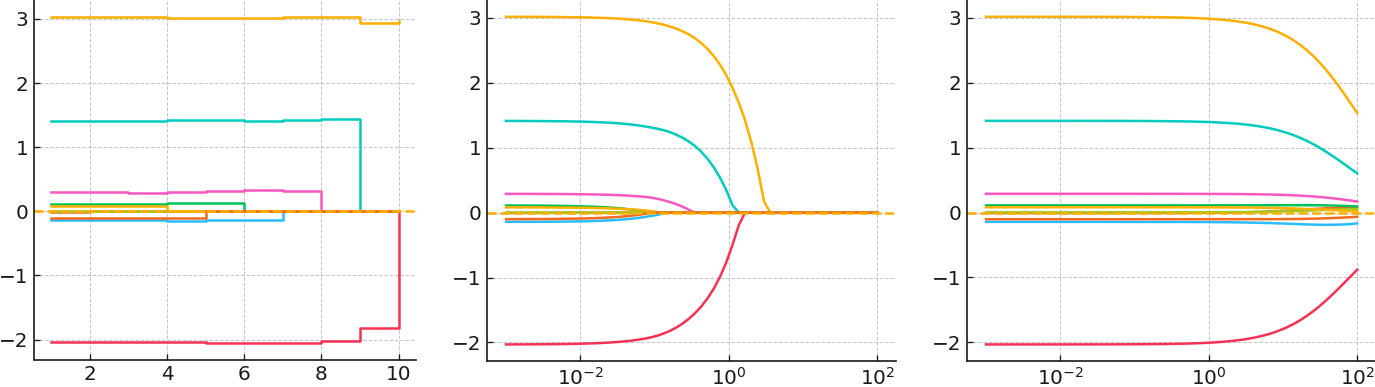
\includegraphics[width=0.98\columnwidth]{images/regularization_path_trim.png}
\end{center}
\begin{center}
    \textbf{Unit Balls of $\ell_p$ Norms in $\mathbb{R}^2$ for Varying $p$:}
    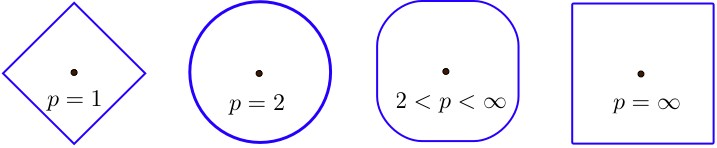
\includegraphics[width=0.9\columnwidth]{images/unit_balls.jpg}
\end{center}

\subsection{Hyperparameter Tuning}
\begin{itemize}
    \item \textbf{K-Fold Cross-Validation:}
\end{itemize}